\chapter{Modelling} \label{chp:models}
    \section{Absorption}
        A critical property of LSP is its ability to absorb laser radiation

        \begin{figure}[h]
            \centering
            \begin{subfigure}[t]{2.6in}
                \centering
                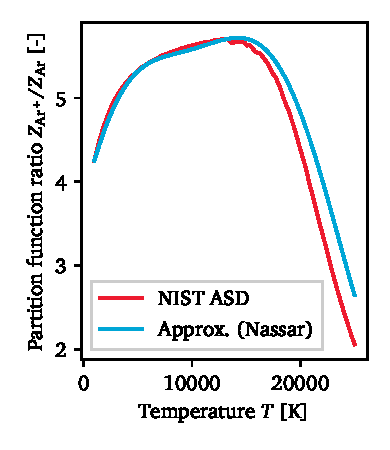
\includegraphics[]{assets/4 models/partition.pdf}
                \caption{Ratio of Ar II to Ar I partition function values}
                \label{fig:e_density_partition}
            \end{subfigure}
            \hfill
            \begin{subfigure}[t]{3.2in}
                \centering
                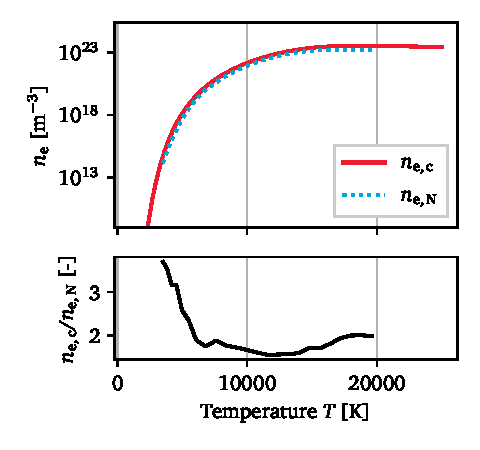
\includegraphics[]{assets/4 models/n_e.pdf}
                \caption{$n_e$ at \qty{1}{bar}, and comparison between computed density $n_\mathrm{e, c}$ and density reported by \textcite{nassarInvestigationLasersustainedPlasma2012} $n_\mathrm{e, N}$}
                \label{fig:e_density_curves}
            \end{subfigure}
            \caption{Computation of electron density $n_e$ of Argon}
            \label{fig:e_density}
        \end{figure}

        \begin{figure}[h]
            \centering
            \begin{subfigure}[t]{2.9in}
                \centering
                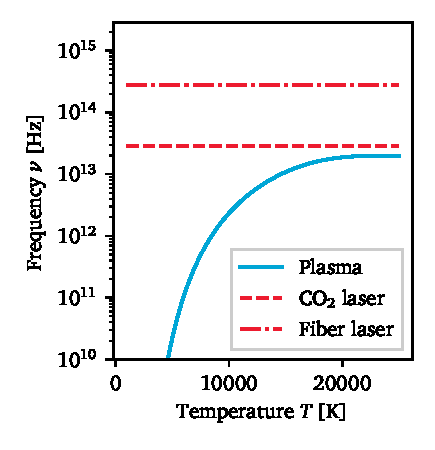
\includegraphics[]{assets/4 models/frequency_comparison.pdf}
                \caption{Comparison of plasma frequency to laser frequency, \qty{10}{bar}}
                \label{fig:coulomb_freq}
            \end{subfigure}
            \hfill
            \begin{subfigure}[t]{2.9in}
                \centering
                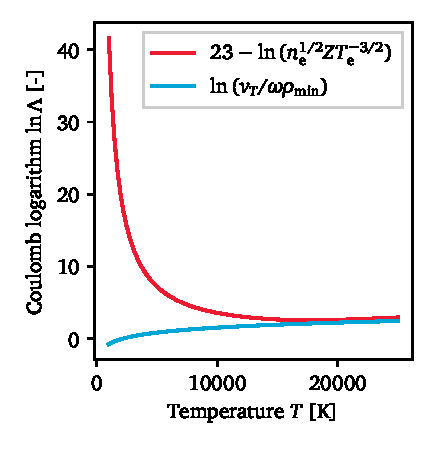
\includegraphics[]{assets/4 models/coulombLog.pdf}
                \caption{Comparison of computation methods for the Coulomb logarithm}
                \label{fig:coulomb_coulomb}
            \end{subfigure}
            \caption{Calculation of the Coulomb logarithm}
            \label{fig:coulomb}
        \end{figure}

        \begin{figure}[h]
            \centering
            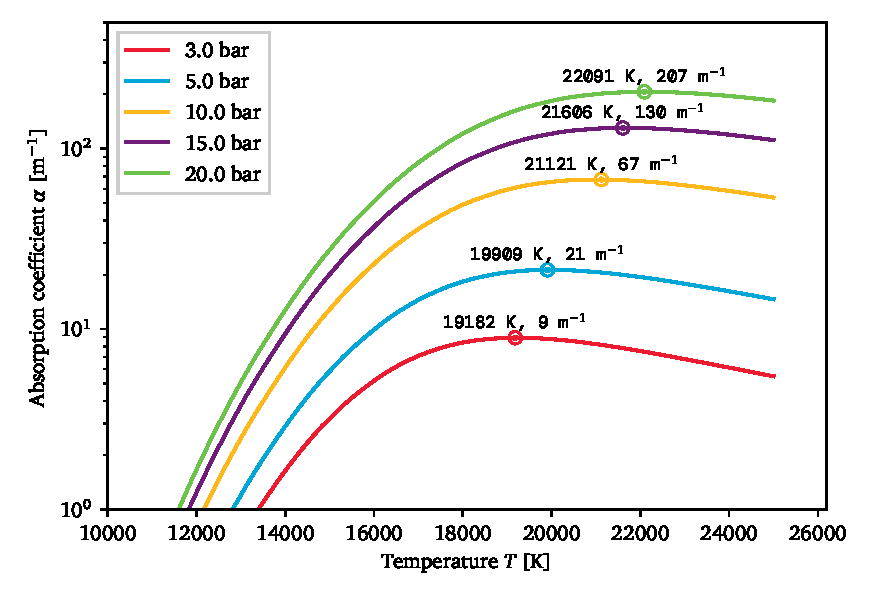
\includegraphics[]{assets/4 models/absorption.pdf}
            \caption{Inverse-brehmsstrahlung absorption coefficient of Argon at various pressures}
            \label{fig:ib_coeff}
        \end{figure}